\documentclass{report}
\usepackage[T1]{fontenc} % Fontes T1
\usepackage[utf8]{inputenc} % Input UTF8
\usepackage[backend=biber, style=ieee]{biblatex} % para usar bibliografia
\usepackage{csquotes}
\usepackage[portuguese]{babel} %Usar língua portuguesa
\usepackage{blindtext} % Gerar texto automaticamente
\usepackage[printonlyused]{acronym}
\usepackage{hyperref} % para autoref
\usepackage{graphicx}
\usepackage{amsmath} % matemática
\usepackage{amssymb} % matemática
\usepackage{float}

\addbibresource{bibliografia.bib}

\begin{document}
%%
% Definições
%
\def\titulo{Trabalho de Aprofundamento 2, Grupo 27}
\def\data{30 de maio de 2021}
\def\autores{Alexandre Martins, Luís Silva}
\def\autorescontactos{(103552) alexandremartins@ua.pt, (103617) afonsotorres@ua.pt}
\def\versao{1}
\def\departamento{DETI}
\def\empresa{Universidade de Aveiro}
\def\logotipo{ua.pdf}
%
%%%%%% CAPA %%%%%%
%
\begin{titlepage}

\begin{center}
%
\vspace*{50mm}
%
{\Huge \titulo}\\ 
%
\vspace{10mm}
%
{\Large \empresa}\\
%
\vspace{10mm}
%
{\LARGE \autores}\\ 
%
\vspace{30mm}
%
\begin{figure}[h]
\center

\includegraphics{\logotipo}
\end{figure}%
\vspace{30mm}
\end{center}
%
\begin{flushright}
\versao
\end{flushright}
\end{titlepage}

%%  Página de Título %%
\title{%
{\Huge\textbf{\titulo}}\\
{\Large \departamento\\ \empresa}
}
%
\author{%
    \autores \\
    \autorescontactos
}
%
\date{\data}
%
\maketitle

\pagenumbering{roman}

%%%%%% Agradecimentos %%%%%%
% Segundo glisc deveria aparecer após conclusão...
\renewcommand{\abstractname}{Agradecimentos}
\begin{abstract}
Gostaríamos de agradecer a: 

\begin{description}
	\item[Professor António Manuel Adrego da Rocha], pelas aulas esclarecedoras que nos foram dadas sobre \LaTeX no semestre passado, sem as quais não conseguiríamos ter completado este relatório e pelas aulas em python, linguagem na qual o trabalho foi realizado, e extensão do prazo de entrega.
	
		\item[João Rodrigo Faria (103361)], pelo pequeno mas relevante apoio que foi dado em \LaTeX na estrutura do relatório. 
	

	
	
	
\end{description}
\end{abstract}


\tableofcontents
\listoffigures


%%%%%%%%%%%%%%%%%%%%%%%%%%%%%%%
\clearpage
\pagenumbering{arabic}

%%%%%%%%%%%%%%%%%%%%%%%%%%%%%%%%%
%%%%%%%%%%%%%%%%%%%%%%%%%%%%%%%%%

\chapter{Introdução}
\label{chap.introducao}

Este trabalho, desenvolvido no âmbito da \ac{uc} de Laboratórios de Informática, consistiu na criação de um servidor que suporte a geração de um número inteiro
aleatório (entre 0 e 100), designado por número secreto, bem como o número
máximo de tentativas (entre 10 e 30) concedidas para o adivinhar. E um cliente que
permita adivinhar esse número secreto. Ou seja um jogo de adivinha o número secreto.\newline
\hfill


O projeto do code.ua associado a este trabalho pode ser consultado em \url{http://code.ua.pt/projects/labi2021-ap2-g27/files}

%%%%%%%%%%%%%%%%%%%%%%%%%%%%%%%%%
%%%%%%%%%%%%%%%%%%%%%%%%%%%%%%%%%

\chapter{Metodologia}
\label{chap.metodologia}
Exposição da metodologia utilizada para a realização do projeto e obtenção de resultados.

%%%%%%%%%%%%%%%%%%%%%%%%%%%%%%%%%

\section{client.py}

\subsection{Objetivos}
O \textbf{client} contacta o servidor para dar início ao jogo (operação \textbf{START)} enviando
um dicionário com o seguinte formato:
\newline

\{"op": "START", "client \textunderscore id": nome identificador do cliente\}
\newline

Após a inicialização do jogo com \textbf{START} o jogador tem 3 opções, \textbf{QUIT}, \textbf{GUESS}, \textbf{STOP}:
\newline
	
\begin{itemize}
	\item \textbf{QUIT} 
\end{itemize}
O cliente contacta o servidor para desistir do jogo enviando um dicionário com o seguinte formato:
 \{ "op": "QUIT" \}


\begin{itemize}
	\item \textbf{GUESS}
\end{itemize}
O cliente contacta o servidor para fazer uma jogada enviando um dicionário com o seguinte formato:
 \{ "op": "GUESS", "number": valor numérico entre 0 e 100\}


\begin{itemize}
	\item \textbf{STOP}

\end{itemize}
O cliente contacta o servidor para terminar o jogo (operação STOP) enviando um
dicionário com o seguinte formato:
\{ "op": "STOP","number": último valor, "attempts": jogadas efectuadas \}


\subsection{Métodos}
\begin{itemize}
 \item \textbf{run\textunderscore client()}
\end{itemize}
Recebe as acções do jogador e processa o jogo.

\begin{itemize}
 \item \textbf{ quit\textunderscore action()}

\end{itemize}
Desiste do jogo, caso se verifiquem as condições necessárias para o fazer.

\begin{itemize}
 \item \textbf{ validate\textunderscore response()} 

\end{itemize}
Verifica se a resposta do servidor é válida.

%%%%%%%%%%%%%%%%%%%%%%%%%%%%%%%%%


\section{server.py}

\subsection{Objetivos}
O ficheiro \textbf{server.py} consiste num conjunto de métodos essenciais para a conexão e troca de mensagens com o servidor remoto.
\newline
\begin{itemize}
	\item \textbf{START}
\end{itemize}
Após o comando \textbf{START} o servidor só deverá aceitar o cliente caso ele não esteja já inscrito na lista de clientes ativos do servidor. Nesse caso gera um número aleatório entre 0 e 100, um número máximo aleatório de jogadas entre 10 e 30 e inicializa o número de
jogadas. Depois deve acrescentar este registo de cliente à sua estrutura de dados
de clientes ativos (para posteriormente evitar a inscrição de outro cliente com a
mesma identificação) e devolve um dicionário indicando que a operação de registo
deste cliente foi feita com sucesso e indicando-lhe quantas jogadas ele dispõe (de
maneira a ele poder controlar o seu jogo) com o seguinte formato:
\newline

\{"op":"START","status": True, "max\textunderscore attempts": nº máximo de jogadas\}
\newline

Se pelo contrário um cliente com o mesmo identificador já se encontra a jogar então
devolve-lhe um dicionário indicando que a operação de registo deste cliente não
teve sucesso com o seguinte formato:
\newline

\{ "op": "START", "status": False, "error": "Cliente existente"\} 
\begin{itemize}
	\item \textbf{QUIT}
\end{itemize}
O servidor só deverá aceitar a desistência do jogador caso ele esteja presentemente
ativo. Nesse caso atualiza o ficheiro de resultados com os dados do cliente e o
resultado indicando a sua desistência ("\textbf{QUIT}"), remove o registo de cliente da sua estrutura de dados de clientes ativos (para posteriormente aceitar a inscrição de
outro cliente com a mesma identificação) e devolve um dicionário indicando que a
operação de desistência deste cliente foi feita com sucesso com o seguinte formato:
\newline

\{"op": "QUIT", "status": True\}
\newline

Se pelo contrário o cliente não está presentemente a jogar então devolve-lhe um
dicionário indicando que a operação de desistência deste cliente não teve sucesso
com o seguinte formato:
\newline

\{"op": "QUIT", "status": False, "error": "Cliente inexistente"\}


\begin{itemize}
	\item \textbf{GUESS}
\end{itemize}
O servidor só deverá aceitar a jogada do cliente caso ele já esteja inscrito na lista de clientes ativos do servidor. Nesse caso contabiliza essa jogada do cliente, compara
o valor indicado pelo cliente com o número secreto. Se o valor indicado pelo cliente
for maior do que o número secreto o servidor indica que na próxima jogada deve
tentar um valor menor ("smaller"). Se pelo contrário o valor indicado pelo cliente
for menor do que o número secreto o servidor indica que na próxima jogada deve
tentar um valor maior ("larger"). Se o cliente acertou então o servidor indica que
os valores são iguais ("equals"). O servidor envia ao cliente um dicionário com o
seguinte formato:
\newline

\{"op": "GUESS", "status": True, "result": "smaller"/"larger"/"equals"\}
\newline

Se pelo contrário o cliente não está presentemente a jogar então devolve-lhe um
dicionário indicando que a operação de adivinhação deste cliente não teve sucesso
com o seguinte formato:
\newline

\{"op": "GUESS", "status": False, "error": "Cliente inexistente"\}



\begin{itemize}
	\item \textbf{STOP}
\end{itemize}

O servidor só deverá aceitar a terminação do jogo caso o jogador esteja presentemente ativo. Nesse caso o servidor verifica se o número de jogadas indicadas pelo
cliente é igual à sua própria contagem. Se o jogador indicar um número correto
de jogadas então o servidor deve verificar o número recebido. Se ele for igual
ao número secreto que o cliente devia adivinhar - e se o cliente não excedeu o
número máximo de jogadas - então o resultado do jogo é de sucesso ("SUCCESS")
caso contrário é de insucesso ("FAILURE"). Depois o servidor atualiza o ficheiro
report.csv com os dados do cliente e o resultado indicando sucesso ou insucesso,
remove o registo de cliente da sua estrutura de dados de clientes ativos (para
posteriormente aceitar a inscrição de outro cliente com a mesma identificação) e
devolve um dicionário indicando que a operação de terminação deste cliente foi
feita com sucesso e indica-lhe qual era o número secreto com o seguinte formato:
\newline

\{"op": "STOP", "status": True, "guess": número secreto\}
\newline

Quando o cliente recebe esta informação do servidor escreve no monitor uma mensagem a indicar se adivinhou ou não o número secreto e quantos jogadas efectuou.
\newline

Se pelo contrário o cliente não está presentemente a jogar ou enviou uma contagem
de jogadas inconsistente o servidor devolve-lhe um dicionário indicando que a operação de terminação não teve sucesso e indicando o erro de "Cliente inexistente" ou
de "Número de jogadas inconsistente", com o seguinte formato:
\newline

\{"op": "QUIT", "status": False, "error": um dos erros indicados em cima\}



\subsection{Métodos}
\begin{itemize}
	\item \textbf{main()}
\end{itemize}


Este método contem a lógica principal de todo o projeto.
É este que é chamado quando se executa o programa.
Pode ser dividido em duas partes:

- Estabelecimento de conexão (encriptada) com o servidor.\newline

- Receção e utilização contínua dos dados recebidos.\newline

\begin{itemize}
	\item \textbf{find\textunderscore client\textunderscore id()}
\end{itemize}
Devolve o ID do utilizador através do socket.

\begin{itemize}
	\item \textbf{new\textunderscore msg()}
\end{itemize}
 Recebe as ações do client.
 
\begin{itemize}
	\item \textbf {new\textunderscore client()}
\end{itemize}
 Gera um novo objecto relativo ao cliente ao qual é atribuído um socket.

\begin{itemize}
	\item \textbf {clean\textunderscore client() e quit\textunderscore client()}
\end{itemize}
Removem um client que for especificado do dicionário global.

\begin{itemize}
	\item \textbf {create\textunderscore file() e update\textunderscore file()}
\end{itemize}
Encarregadas de gerar e atualizar os ficheiros CSV.


\begin{itemize}
	\item \textbf {guess\textunderscore client()}
\end{itemize}
Compara o valor introduzido pelo utilizador ao valor do número secreto registado no dicionário global e devolve uma string relativa à comparação dos dois.

\begin{itemize}
	\item \textbf {stop\textunderscore client()}
\end{itemize}
Atualiza o ficheiro CSV com o resultado do jogo.


%%%%%%%%%%%%%%%%%%%%%%%%%%%%%%%%%

\section{Segurança}
\subsection{Contexto}

%%%%%%%%%%%%%%%%%%%%%%%%%%%%%%%%%%%%%%%%%%%%%%%%%%%%%%%%%%%%%%%%%

\subsubsection{Troca do segredo partilhado}
A troca de chaves Diffie Hellman é um método de troca segura de chaves criptográficas em um canal público e foi um dos primeiros protocolos de chave pública concebidos por Ralph Merkle e nomeados em homenagem a Whitfield Diffie e Martin Hellman. DH é um dos primeiros exemplos práticos de troca de chave pública implementada no campo da criptografia. \newline
O método de troca de chave Diffie – Hellman permite que duas partes que não têm conhecimento prévio uma da outra estabeleçam em conjunto uma chave secreta compartilhada em um canal inseguro. Essa chave pode então ser usada para criptografar comunicações subsequentes usando uma cifra de chave simétrica.

\subsubsection{Encriptação}
Após ser gerado o segredo, é possível agora a \textbf{cifra das mensagens}, para que assegure um nível relativamente satisfatório de segurança.

%%%%%%%%%%%%%%%%%%%%%%%%%%%%%%%%%%%%%%%%%%%%%%%%%%%%%%%%%%%%%%%%%

%%%%%%%%%%%%%%%%%%%%%%%%%%%%%%%%%

\chapter{Testes}
\label{chap.testes}

Para o fazer, primeiro foram declaradas diversas variáveis com strings válidas e inválidas, e, para cada string válida, um dicionário correspondente (para comparar com o resultado de com a string usada como argumento).\newline


Não foram feitos testes unitários para as restantes funções visto que essas dependiam de comunicação com o servidor.




%%%%%%%%%%%%%%%%%%%%%%%%%%%%%%%%%

\chapter{Conclusões}
\label{chap.conclusao}
\section{Resultados}
No que toca aos resultados obtidos pela execução do programa, este funciona corretamente.\newline

Como mostra a imagem 4.1, observa-se que os dados que são enviados pelo servidor são corretamente impressos no terminal.

\begin{figure}[h]
\center
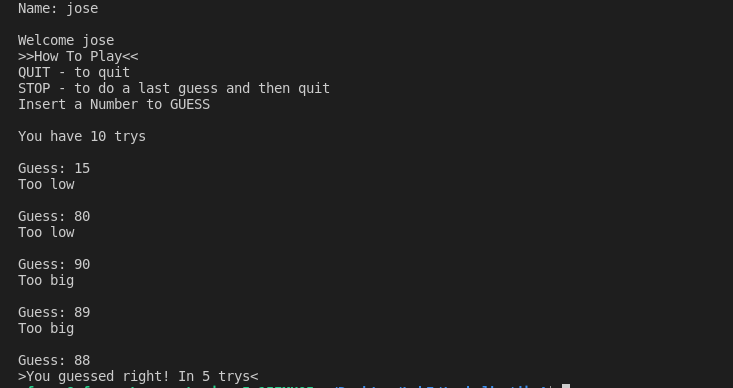
\includegraphics[scale=0.49]{teste1}
\label{pog}
\caption{Simulação da tentativa de um jogador chamado jose}
\end{figure}

Na imagem 4.2 está representada uma simulação do que aconteceria se um jogador escolhesse fazer \textbf{STOP}
\begin{figure}[h]
\center
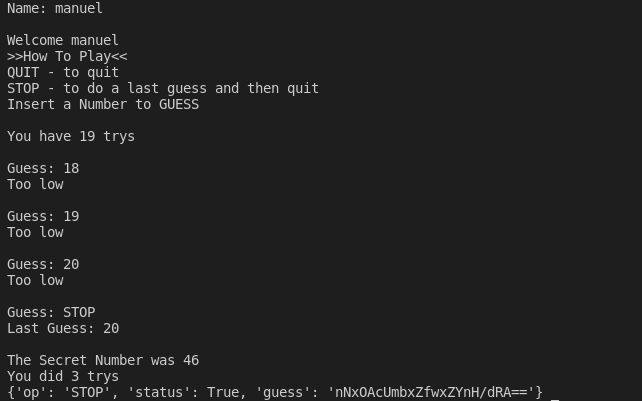
\includegraphics[scale=0.49]{teste2stop}
\label{pog}
\caption{Exemplo da utilização de \textbf{STOP}}
\end{figure}

Na imagem 4.3 está representada uma simulação do que aconteceria se um jogador escolhesse fazer \textbf{QUIT}

\begin{figure}[h]
\center
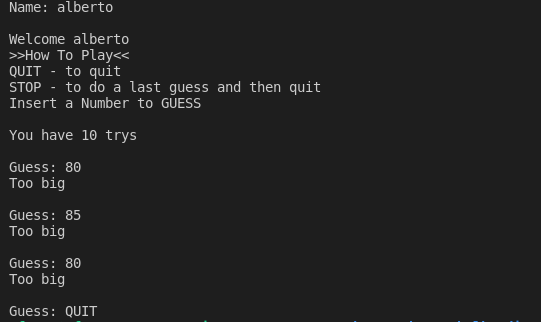
\includegraphics[scale=0.49]{teste3quit}
\label{pog}
\caption{Exemplo da utilização de \textbf{QUIT}}
\end{figure}

\section{Conclusão}
Este trabalho de aprofundamento permitiu aos autores do mesmo consolidar a implementação de sockets, manipulação de estruturas de ficheiros ou mensagens na linguagem de programação Python. Para além disso, forneceu uma ideia geral na negociação de um segredo partilhado pelo método de Diffie-Hellmann.

\chapter*{Contribuições dos autores}
A contribuição de ambos os membros para o bom funcionamento do grupo e projeto foi igual, isto é 50\% 50\%.

%%%%%%%%%%%%%%%%%%%%%%%%%%%%%%%%%
\chapter*{Acrónimos}
\begin{acronym}
\acro{dh}[DH]{Diffie-Hellmann}
\acro{uc}[UC]{Unidade Curricular}
\end{acronym}


%%%%%%%%%%%%%%%%%%%%%%%%%%%%%%%%%
\chapter{Bibliografia}


 \href{https://elearning.ua.pt/pluginfile.php/430960/mod_resource/content/13/ap2-2021.pdf}{Enunciado utilizado na criação do projeto, do qual foram retirados definições de funções e partes do código.}
 \newline
 
 \href{https://en.wikipedia.org/wiki/Cryptography}{Pagina utilizada para melhor compreender o conceito de criptografia.}


\printbibliography

\end{document}
